% =====================================================================
\chapter{Noticias, sentimiento y mercado: el caso del S\&P~Merval}
\chaptermark{Noticias, sentimiento y mercado}
\label{cap:marco}

Que «las noticias mueven la bolsa» es una frase que mezcla dos ideas. La primera es que el
precio de una acción resume lo que los inversores saben y esperan de la empresa, y que cambia
cuando llega información nueva. La segunda es que los medios son el vehículo de esa
información. Si las dos son ciertas, una noticia relevante debería mover el precio en cuanto
se publica. Pero los medios también cumplen otra función: informan sobre el propio mercado.
Una nota que cuenta que «el Merval subió 5\%» es una noticia económica con tono positivo, y
su causa es el precio, no al revés. Este capítulo presenta los conceptos con los que se
analiza esa doble relación y describe el mercado argentino en el período estudiado.

% ---------------------------------------------------------------------
\section{Conceptos centrales}
\label{sec:conceptos}

\subsection{Shock informativo}

Se llama \textit{shock informativo} a la llegada de información que se aparta de lo esperado
y que, por eso, puede cambiar las expectativas de los inversores. El plan de trabajo lo define
por la cantidad: un aumento anormal del volumen de noticias publicadas, medido con un puntaje
$z$ respecto de la media de los 30 días previos. En este trabajo se usa además una definición
por el tono: días en que las noticias son mucho más positivas o negativas que lo habitual. Las
dos definiciones miden cosas distintas. La cantidad capta la \textit{atención}, cuánto se habla
de un tema o de una empresa \citep{da2011,fang2009,cao2025hype}; el tono capta el
\textit{contenido}, si lo que se dice es bueno o malo \citep{tetlock2007,ardia2022}.

\subsection{Eficiencia de mercado}

La hipótesis de mercados eficientes \citep{fama1970} sostiene que los precios reflejan toda
la información disponible. En su versión semifuerte, la información pública, como una
noticia, se incorpora al precio tan rápido que no se puede usar para anticiparlo. Si el
mercado argentino fuera eficiente en ese sentido, el tono de las noticias no debería anticipar
los retornos de los días siguientes: cualquier efecto quedaría en la misma rueda en que la
noticia se conoce. Una consecuencia de la eficiencia es que el precio sigue un paseo aleatorio
y el retorno no tiene tendencia, lo que se prueba con tests de raíz unitaria. La evidencia
para Argentina y la región es mixta: \citet{zablotsky2002} discute la eficiencia del mercado
de capitales argentino, \citet{worthington2003} rechazan el paseo aleatorio en siete bolsas
latinoamericanas y \citet{medina2013} revisa la hipótesis en los principales mercados de la
región. En otros mercados emergentes la eficiencia también varía según el período
\citep{jain2020,malafeyev2017,kulikova2024,rochafilho2019}.

\subsection{Sentimiento del inversor y tono de los medios}

El sentimiento del inversor es el grado de optimismo o pesimismo que no se explica por los
fundamentos. \citet{tetlock2007} lo midió en el tono de una columna periodística y encontró
que un tono muy pesimista anticipa bajas transitorias de los precios, que se revierten: un
efecto de sentimiento y no de información. \citet{garcia2013} mostró que ese efecto se
concentra en las recesiones, cuando los inversores están más atentos a las malas noticias.
Que el tono sea un \textit{reflejo} del mercado también tiene respaldo: en
\citet{tetlock2007} los retornos bajos anticipan columnas más pesimistas, y \citet{verma2026}
encuentran, para el shock de 2020, que buena parte de la cobertura refleja información que el
precio ya había incorporado.

\subsection{Causalidad de Granger y modelos VAR}

Con datos observacionales no se puede probar una causa en sentido estricto, pero sí qué
variable se mueve antes. Una variable $X$ \textit{causa en sentido de Granger} a otra $Y$ si
el pasado de $X$ mejora la predicción de $Y$ más allá de lo que predice el propio pasado de
$Y$ \citep{granger1969}. La prueba se hace dentro de un modelo de vector autorregresivo (VAR),
que explica cada variable con los rezagos de todas \citep{sims1980,lutkepohl2005}. El VAR
permite además simular cómo responde cada variable a un «golpe» en otra (funciones de
impulso-respuesta). Es el marco natural para la pregunta de esta tesina, porque trata las dos
direcciones —noticias \flecha{} mercado y mercado \flecha{} noticias— de forma simétrica.

\subsection{Estudios de eventos}

Un estudio de eventos mide qué hace el precio alrededor de un hecho puntual, comparado con lo
que habría sido normal \citep{mackinlay1997,brown1985}. Se define una ventana de estimación,
donde se calcula el retorno «normal», y una ventana del evento, donde se mide el retorno
\textit{anormal}: lo que el precio se movió de más o de menos. Si una noticia mueve el
mercado, el retorno anormal aparece el día del evento o después; si la noticia refleja lo que
el mercado ya hizo, aparece antes. En Argentina, \citet{calandroni2026} aplicó este método a
las elecciones nacionales entre 2011 y 2023.

\subsection{Volatilidad y regímenes de mercado}

La volatilidad de los mercados no es constante: se agrupa en períodos de calma y de estrés.
Para el S\&P~Merval esto está documentado con modelos de la familia GARCH
\citep{segovia2022,segovia2022wp,larre2019,xenofontos2014}, que además muestran que las
caídas aumentan la volatilidad más que las subas \citep{otuki2008}. Una forma de describir esa
alternancia es suponer que el mercado pasa por un número finito de \textit{regímenes}, cada uno
con su nivel de volatilidad, y que salta de uno a otro según una cadena de Markov
\citep{hamilton1989,rabiner1989,kim1994}. Para mercados latinoamericanos,
\citet{ataurima2016} y \citet{caballero2016} estiman modelos de cambio de régimen sobre
acciones y tipo de cambio, y trabajos recientes los usan para pronosticar volatilidad
\citep{blake2025,ataei2025} o armar carteras \citep{majumder2023}. El régimen importa para esta
tesina porque la relación entre noticias y precios podría cambiar según el mercado esté calmo o
tenso \citep{garcia2013}.

\begin{table}[H]
\centering\small
\begin{tabularx}{\linewidth}{@{}L{2.8cm}YY@{}}
\toprule
 & \textbf{Noticias \flecha{} mercado} & \textbf{Mercado \flecha{} noticias} \\
\midrule
Mecanismo & La nota trae información nueva o mueve el ánimo de los inversores & La nota cuenta lo que el mercado ya hizo \\
Qué se espera ver & El tono anticipa el retorno o el volumen de las ruedas siguientes & El retorno anticipa el tono de las notas siguientes \\
En un estudio de eventos & El retorno anormal aparece el día del evento o después & El retorno anormal aparece antes del evento \\
Con notas de la noche & El tono de la noche anticipa el salto de apertura & El tono de la noche refleja el cierre del día \\
Referencias & \citet{tetlock2007}, \citet{garcia2013}, \citet{galdi2018} & \citet{tetlock2007}, \citet{verma2026} \\
\bottomrule
\end{tabularx}
\caption{Las dos direcciones de la relación entre noticias y mercado y cómo se reconoce cada
una en los datos. Fuente: elaboración propia.}
\label{tab:mecanismos}
\end{table}

% ---------------------------------------------------------------------
\section{El mercado argentino en la ventana de estudio}
\label{sec:mercado-argentino}

El S\&P~Merval es el índice principal de BYMA y reúne a las acciones más negociadas del
mercado local. Es un mercado chico y con liquidez dispareja: junto a acciones muy operadas,
como YPF o Grupo Financiero Galicia, cotizan empresas que pasan días sin operaciones. Los
precios están en pesos, de modo que su tendencia incluye la inflación y la evolución del tipo
de cambio.

En Argentina no existe un mercado de opciones con la liquidez necesaria para calcular un
índice de volatilidad implícita como el VIX de Chicago. Por eso se construyó un \textit{VIX
argentino} con volatilidad realizada: el desvío estándar de los retornos diarios del índice en
las últimas 20 ruedas, anualizado \citep{sakowski2023}. Entre el 2 de enero de 2025 y el 30
de abril de 2026 (323 ruedas) promedió 44,0\%, con un mínimo de 15,4\% el 30/04/2026 y un
máximo de 91,0\% el 21/11/2025 (figura~\ref{fig:vix}).

\begin{figure}[H]
\centering
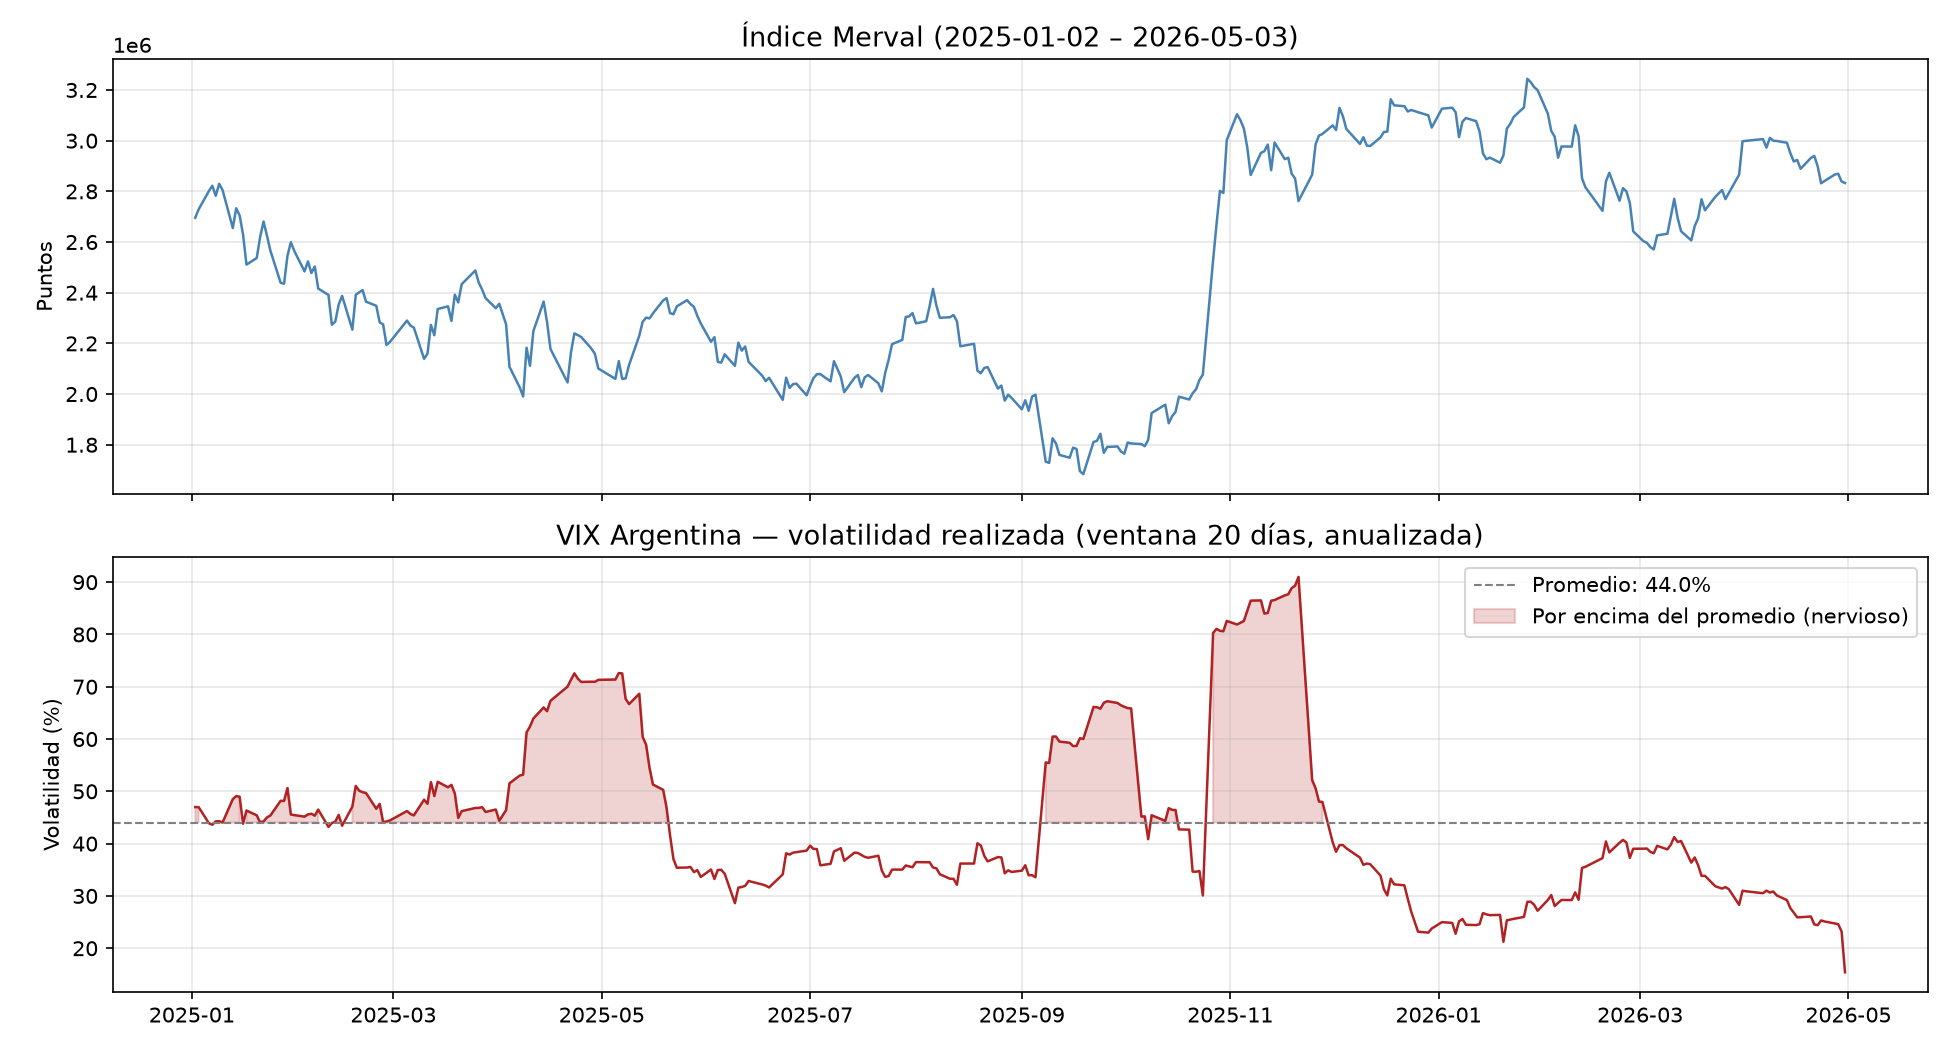
\includegraphics[width=0.95\linewidth]{vix_arg.png}
\caption{S\&P~Merval en pesos (arriba) y VIX argentino (abajo), del 2/1/2025 al 30/4/2026.
El sombreado marca los días por encima del promedio. Fuente: elaboración propia con datos de
Yahoo Finance (\carpeta{Lado Bursatil/03_vix_argentino}).}
\label{fig:vix}
\end{figure}

El período tuvo tres episodios de volatilidad alta, todos disparados por un hecho puntual
(tabla~\ref{tab:episodios}). El primero coincide con la turbulencia global por los aranceles
de Estados Unidos y la salida del cepo cambiario; los otros dos arrancan el día hábil
siguiente a una elección. El máximo de toda la serie no vino de una caída sino de la suba de
21,8\% del 27/10/2025, después de las legislativas nacionales. A estos hechos se suma el
anuncio de apoyo financiero del Tesoro de Estados Unidos del 24/09/2025.

\begin{table}[H]
\centering\small
\begin{tabularx}{\linewidth}{@{}L{3.1cm}C{1.1cm}L{2.6cm}L{2.2cm}Y@{}}
\toprule
\textbf{Período} & \textbf{Ruedas} & \textbf{Pico del VIX} & \textbf{Disparador} & \textbf{Contexto} \\
\midrule
09/04 al 14/05/2025 & 22 & 72,6\% (06/05) & 09/04: +9,7\% & Aranceles de EE.\,UU.; incluye la salida del cepo (14/04) \\
08/09 al 03/10/2025 & 20 & 67,2\% (26/09) & 08/09: $-$13,3\% & Día hábil siguiente a las elecciones bonaerenses (07/09) \\
27/10 al 21/11/2025 & 20 & 91,0\% (21/11) & 27/10: +21,8\% & Día hábil siguiente a las legislativas nacionales (26/10) \\
\bottomrule
\end{tabularx}
\caption{Episodios con el VIX argentino por encima de 55\%. Fuente: elaboración propia
(\carpeta{Lado Bursatil/03_vix_argentino}).}
\label{tab:episodios}
\end{table}

Una advertencia de lectura: como el VIX argentino es un desvío de 20 ruedas, un único día
extremo queda dentro del cálculo durante exactamente 20 ruedas. El índice salta el día del
shock y cae de golpe 20 ruedas después, aunque ese día el mercado no haga nada especial. Los
dos episodios del segundo semestre duran exactamente 20 ruedas: son, casi en su totalidad, el
eco de un único día. Este artefacto de las medias móviles con pesos iguales está descrito en
la literatura como \textit{ghost features} \citep{papaioannou2014}; una media exponencial
\citep{riskmetrics1996} lo atenuaría.

% ---------------------------------------------------------------------
\section{Unidades de análisis}
\label{sec:unidades}

\textbf{Las acciones.} El panel tiene 47 acciones de BYMA, en diez sectores
(tabla~\ref{tab:sectores}). Incluye a las 20 que integran el S\&P~Merval y a 27 más, todas
con cotización en el 100\% de las ruedas de tres años y al menos 90\% de días con volumen real
(sección~\ref{sec:recoleccion}). El listado completo, con la liquidez, la volatilidad y la
cobertura de noticias de cada una, está en el anexo~\ref{anx:panel}.

\begin{table}[H]
\centering\small
\begin{tabular}{@{}lcL{8.6cm}@{}}
\toprule
\textbf{Sector} & \textbf{Acciones} & \textbf{Tickers} \\
\midrule
Consumo & 9 & GRIM, HAVA, LEDE, LONG, MIRG, MOLI, MORI, SAMI, SEMI \\
Financiero & 8 & BBAR, BHIP, BMA, BPAT, BYMA, GGAL, SUPV, VALO \\
Utilities & 8 & CEPU, CGPA2, DGCU2, EDN, GBAN, METR, PAMP, TRAN \\
Materiales & 6 & ALUA, CELU, FIPL, LOMA, RIGO, TXAR \\
Energía & 4 & CAPX, TGNO4, TGSU2, YPFD \\
Conglomerado & 3 & COME, CRES, GARO \\
Industrial & 3 & AGRO, AUSO, OEST \\
Real Estate & 3 & CTIO, GCDI, IRSA \\
Comunicaciones & 2 & CVH, TECO2 \\
Tecnología & 1 & BOLT \\
\midrule
\textbf{Total} & \textbf{47} & \\
\bottomrule
\end{tabular}
\caption{Panel de acciones por sector. Fuente: elaboración propia
(\carpeta{Lado Bursatil/01_scraping_acciones}).}
\label{tab:sectores}
\end{table}

\textbf{Las empresas con tono propio.} No todas las empresas aparecen seguido en las noticias.
Para medir el tono propio de una empresa hace falta que tenga noticias en buena parte de las
ruedas; con un corte de 90 de las 244 ruedas quedan 17: YPFD, BBAR, SUPV, EDN, GGAL, CEPU,
TGSU2, IRSA, BMA, LOMA, PAMP, CRES, BYMA, TRAN, METR, TXAR y ALUA. Cualquier corte entre 75 y
94 ruedas da exactamente las mismas 17. Las otras 30 entran a los modelos con el tono general
del mercado.

\textbf{Los portales.} El corpus reúne siete portales nacionales, recolectados en nueve
fuentes (tabla~\ref{tab:corpus}). iProfesional aporta el 39\% de las notas y Clarín el 29\%;
TN es el más chico. Cada portal tiene su propio tono promedio, de +30,4 puntos en TN a 0,0 en
Ámbito Finanzas, lo que obliga a controlar la composición por portal cuando se arma la serie
diaria (sección~\ref{sec:tono-rueda}).

\begin{table}[H]
\centering\small
\begin{tabular}{@{}llr@{}}
\toprule
\textbf{Portal} & \textbf{Método de recolección} & \textbf{Artículos} \\
\midrule
iProfesional & Mapa del sitio & 5.455 \\
Clarín & Mapa del sitio & 3.737 \\
Clarín — Economía & Wayback Machine & 294 \\
El Economista & Mapa del sitio & 2.695 \\
Ámbito Financiero — Economía & Wayback Machine & 498 \\
Ámbito Financiero — Finanzas & Wayback Machine & 240 \\
Infobae — Economía & Wayback Machine & 500 \\
La Nación — Economía & Wayback Machine & 491 \\
TN — Economía & Wayback Machine & 102 \\
\midrule
\textbf{Total} & & \textbf{14.012} \\
\bottomrule
\end{tabular}
\caption{Corpus de noticias por fuente, después de la depuración. Fuente: elaboración propia
(\carpeta{Lado Noticias/noticias}).}
\label{tab:corpus}
\end{table}
